%beamer

%\PassOptionsToClass{handout}{beamer}

% \newboolean{handoutmode}
% \setboolean{handoutmode}{false}
%\newcommand{\handoutmode}{}

%% LaTeX-Beamer template for KIT design
%% by Erik Burger, Christian Hammer
%% title picture by Klaus Krogmann
%%
%% version 2.1
%%
%% mostly compatible to KIT corporate design v2.0
%% http://intranet.kit.edu/gestaltungsrichtlinien.php
%%
%% Problems, bugs and comments to
%% burger@kit.edu
\ifdefined \handoutmode
\documentclass[18pt, handout]{beamer}
\else
\documentclass[18pt]{beamer}
\fi

\usepackage[T1]{fontenc}
\usepackage[utf8]{inputenc}

\usepackage{../preamble/templates/beamerthemekit}

\usepackage[vlined]{algorithm2e}  %possible: noend, noline, ...
\usepackage{amssymb}
\usepackage{amsmath}
\usepackage{wasysym}
\usepackage{graphicx}
%\usepackage{hyperref}
\usepackage[export]{adjustbox}
\usepackage{wrapfig}
\usepackage{colortbl}
\usepackage{tikz}
\usetikzlibrary{matrix}
\usetikzlibrary{arrows.meta}
\usetikzlibrary{automata}
\usetikzlibrary{tikzmark}
\graphicspath{{images/}}
%\usepackage[colorlinks=true,urlcolor=blue,linkcolor=blue]{hyperref}
\usepackage[outline]{contour}
\usepackage{cancel}
\usepackage[warn]{textcomp}
\usepackage{multicol}
\usepackage{tabularx}
\usepackage{xcolor}
\usepackage{hhline}
\usepackage{environ}
\usepackage{calc}
\usepackage{bm}
\usepackage{xspace} % for \xspace command
\usepackage{varwidth}
\usepackage{csquotes}

\newcommand{\mycomment}[1]{}

%%%% CONFIG

\input{../preamble/config.tex}

%%%% CONFIG END

%\renewcommand{\SS}{\iffontchar\font"1E9E \symbol{"1E9E}\else SS\fi} % SHAME ON YOU, LATEX!
\newcommand{\TM}{\text{$\mbox{}^\text{\tiny TM}$}}
\newcommand{\pluseq}{\mathrel{+}=}
\newcommand{\pp}{\operatorname{++}} 
\newcommand{\mm}{\operatorname{--\mbox{\:}--}}
\newcommand{\minuseq}{\mathrel{-}=}
\newcommand{\asteq}{\mathrel{*}=}
\newcommand{\muleq}{\asteq}
\renewcommand{\mod}{\mathop{\textbf{mod}}} 
\renewcommand{\div}{\mathop{\textbf{div}}}
\newcommand{\N}{\mathbb{N}} 
\newcommand{\R}{\mathbb{R}}
\newcommand{\Z}{\mathbb{Z}}
\newcommand{\E}{\mathbb{E}}
\renewcommand{\P}{\mathbb{P}}
\newcommand{\BB}{\mathbb{B}} % \B already exists
\newcommand{\NP}{\ensuremath{\mathcal{N\hspace{-1.5pt}P}}}
\newcommand{\Oh}[1]{\mathcal{O}\!\left(#1\right)}
\renewcommand{\O}{\mathcal{O}}
\newcommand{\Om}[1]{\Omega\!\left(#1\right)}
\newcommand{\Th}[1]{\Theta\!\left(#1\right)}

\newcommand{\realTilde}{\textasciitilde\xspace}
\renewcommand{\qedsymbol}{\textcolor{black}{\openbox}}

\newcommand{\size}[1]{\ensuremath{\left\lvert #1 \right\rvert}}
\newcommand{\set}[1]{\left\{#1\right\}}
\newcommand{\tuple}[1]{\left(#1\right)}

\newcommand*{\from}{\colon}

\newcommand{\morescalingdelimiters}{   % for proper \left( \right) typography
	\delimitershortfall=0pt  % formerly: 0pt  
	\delimiterfactor=1
}
% todo later
%\delimitershortfall=0pt  % for proper \left( \right) typography
%\delimiterfactor=1

% --- \frameheight constant ---
\newlength\fullframeheight
\newlength\framewithtitleheight
\setlength\fullframeheight{.92\textheight}
\setlength\framewithtitleheight{.86\textheight}

\newlength\frameheight
\setlength\frameheight{\fullframeheight}

\let\frametitleentry\relax
\let\oldframetitle\frametitle
\def\frametitle#1{\global\def\frametitleentry{#1}\if\relax\frametitleentry\relax\else\setlength\frameheight{\framewithtitleheight}\fi\oldframetitle{#1}}

% --- \frameheight constant end ---

\def\·{\cdot}
\def\*{\cdot}
\def\<{\langle}
\def\>{\rangle}


\newcommand{\zB}{z.\,B.\@\xspace}
\newcommand{\ZB}{Z.\,B.\@\xspace}

\newcommand{\ceil}[1]{\left\lceil#1\right\rceil}
\newcommand{\floor}[1]{\left\lfloor#1\right\rfloor}
\newcommand{\abs}[1]{\left|#1\right|}
\newcommand{\Matrix}[1]{\begin{pmatrix} #1 \end{pmatrix}}
\newcommand{\braced}[1]{\left\lbrace #1 \right\rbrace}
\newcommand{\llist}[1]{\langle #1 \rangle}
\newcommand{\Mid}{\;\middle|\;}

\let\after\circ

\newcommand{\entspr}{\ensuremath{\mathrel{\hat{=}}}\xspace}

\def\~~>{\ensuremath{\rightsquigarrow}}  % FuCKING FINALLY! :D

% "something" placeholder. Useful for repairing spacing of operator sections, like `\sth = 42`.
\def\sth{\vphantom{.}}

\def\fract#1/#2 {\frac{#1}{#2}}  % ! TRAILING SPACE is CRUCIAL!
\def\dfract#1/#2 {\dfrac{#1}{#2}} % ! Trailing space is crucial!

\newcommand{\tight}[1]{{\renewcommand{\arraystretch}{0.76} #1}}
\newcommand{\stackedtight}[1]{{\renewcommand{\arraystretch}{0.76} \begin{matrix} #1 \end{matrix}} }
\newcommand{\stacked}[1]{\begin{matrix} #1 \end{matrix} }
\newcommand{\casesl}[1]{\delimitershortfall=0pt  \left\lbrace\hspace{-.3\baselineskip}\begin{array}{ll} #1 \end{array}\right.}
\newcommand{\casesr}[1]{\delimitershortfall=0pt  \left.\begin{array}{ll} #1 \end{array}\right\rbrace}
\newcommand{\caseslr}[1]{\delimitershortfall=0pt  \left\lbrace\begin{array}{ll} #1 \end{array}\hspace{-.3\baselineskip}\right\rbrace}

\def\q#1uad{\ifnum#1=0\relax\else\quad\q{\the\numexpr#1-1\relax}uad\fi}
% e.g. \q1uad = \quad, \q2uad = \qquad etc.

\newcommand{\qqquad}{\q3uad}


\def\indentstring{}
\def\§#1{\def\indentstring{#1}#1}
\def\.{{$\hphantom{\text{\indentstring}}$}}


\newcommand{\impl}{\ifmmode\ensuremath{\mskip\thinmuskip\Rightarrow\mskip\thinmuskip}\else$\Rightarrow$\xspace\fi}  
\newcommand{\Impl}{\ifmmode\implies\else$\Longrightarrow$\xspace\fi}

\newcommand{\gdw}{\ifmmode\mskip\thickmuskip\Leftrightarrow\mskip\thickmuskip\else$\Leftrightarrow$\xspace\fi}
\newcommand{\Gdw}{\ifmmode\iff\else$\Longleftrightarrow$\xspace\fi}

\newcommand{\symbitemnegoffset}{\hspace{-.33\baselineskip}}
\newcommand{\implitem}{\item[\impl\symbitemnegoffset]}
\newcommand{\Implitem}{\item[\Impl\symbitemnegoffset]}


\newcommand{\forcenewline}{\mbox{}\\}

\newcommand{\bfalert}[1]{\textbf{\alert{#1}}}
\let\elem\in   % I'm a Haskell freak. Don't judge me. :P


\newenvironment{threealign}{%
	\[
	\begin{array}{r@{\ }c@{\ }l}
}{%
	\end{array}	
	\]
}


\makeatletter
% Provides color if undefined.
\newcommand{\colorprovide}[2]{%
	\@ifundefinedcolor{#1}{\colorlet{#1}{#2}}{}}
\makeatother



%\pgfdeclarelayer{background}
%\pgfdeclarelayer{foreground}
%\pgfsetlayers{background,main,foreground}

\colorprovide{lightred}{red!30}
\colorprovide{lightgreen}{green!40}
\colorprovide{lightyellow}{yellow!50}
\colorprovide{beamerlightred}{lightred}
\colorprovide{beamerlightgreen}{lightgreen}
\colorprovide{beamerlightyellow}{lightyellow}
\colorprovide{fullred}{red!60}
\colorprovide{fullgreen}{green}
\definecolor{darkred}{RGB}{115,48,38}
\definecolor{darkgreen}{RGB}{48,115,38}
\definecolor{darkyellow}{RGB}{100,100,0}

\only<handout:0>{\colorlet{adaptinglightred}{beamerlightred}}
\only<handout:0>{\colorlet{adaptinglightgreen}{beamerlightgreen}}
\only<handout:0>{\colorlet{adaptinglightyellow}{beamerlightyellow}}
\only<beamer:0>{\colorlet{adaptinglightred}{lightred}}
\only<beamer:0>{\colorlet{adaptinglightgreen}{lightgreen}}
\only<beamer:0>{\colorlet{adaptinglightyellow}{lightyellow}}
\only<handout:0>{\colorlet{adaptingred}{lightred}}
\only<beamer:0>{\colorlet{adaptingred}{fullred}}
\only<handout:0>{\colorlet{adaptinggreen}{lightgreen}}
\only<beamer:0>{\colorlet{adaptinggreen}{fullgreen}}

\colorlet{checkgreen}{green!80}
\colorlet{crashred}{fullred}
\colorprovide{myalertcolor}{red}
\colorlet{alertcolor}{myalertcolor}

\definecolor{kwblue}{rgb}{0.3,0.3,1}
\definecolor{strcolor}{RGB}{48,115,38}

\newcommand{\str}[1]{\shorthandoff{"}\textcolor{strcolor}{\text{"{}#1"{}}\shorthandon{"}}}

\newcommand{\gray}[1]{\textcolor{gray}{#1}}

\newcommand{\MyKwSty}[1]{\textcolor{kwblue}{\textbf{#1}}}
\SetKwSty{MyKwSty}

\SetArgSty{textnormal} % to end conditional italics madness

\newcommand{\MyCommentSty}[1]{\emph{\gray{#1}}}
\SetCommentSty{MyCommentSty}

\SetKwComment{Comment}{// }{}

\newcommand{\LComment}[1]{\Comment*[h]{#1}}
\newcommand{\RComment}[1]{\quad \Comment*[h]{#1}}



\SetKwBlock{KwFunc}{function}{}
\SetKwBlock{KwProc}{procedure}{}
\newcommand{\Function}[2]{\KwFunc({#1}){#2}}
\newcommand{\Procedure}[2]{\KwProc({#1}){#2}}
\SetKwBlock{KwEmptyBlock}{}{}
\newcommand{\EmptyBlock}[1]{\KwEmptyBlock(){#1}}

% Binary operator keywords (small surrounding spaces)
\newcommand{\SetKwBin}[2]{
	\expandafter\newcommand\csname #1\endcsname{\ensuremath{\mathbin{\KwSty{#2}}}}	
}
% Relational operator keywords (bigger surrounding spaces)
\newcommand{\SetKwRel}[2]{
	\expandafter\newcommand\csname #1\endcsname{\ensuremath{\mathrel{\KwSty{#2}}}}	
}
% Directive keywords (trailing space)
\newcommand{\SetKwDir}[2]{
	\expandafter\newcommand\csname #1\endcsname{\ensuremath{\mathop{\KwSty{#2}}}}		
}

\DontPrintSemicolon
%\SetKwSwitch{Switch}{Case}{Other}{switch on}{}{}{else}{}{}

%\newcommand{\SwitchCase}[2]{\KwSty{case} #1 \KwOf\EmptyBlock{#2}}
%\newcommand{\case}[2]{#1:\EmptyBlock{#2}}
\SetKwDir{KwAssert}{assert}
\SetKwDir{KwInvariant}{invariant}
\SetKwRel{KwStep}{step}
\SetKwRel{KwDownto}{downto}	
\SetKwDir{KwArrayOf}{array of\,}
\SetKwDir{KwArray}{array}
\let\KwTo\undefined
\SetKwRel{KwTo}{to}
\SetKwRel{KwOf}{of}
\let\KwInput\KwIn
\let\KwIn\undefined
\SetKwRel{KwIn}{in}
\SetKwRel{KwInto}{into}
\SetKwDir{KwNot}{not}
\SetKwRel{KwIs}{is}
\SetKwRel{KwAnd}{and}
\SetKwRel{KwOr}{or}
\SetKwBin{KwMod}{mod}
\SetKwBin{KwDiv}{div}
\SetKwDir{KwContinue}{continue}
\SetKwDir{KwBreak}{break}
\SetKwDir{KwThrow}{throw}
\SetKw{KwTrue}{true}
\SetKw{KwFalse}{false}
\SetKw{KwThis}{this}
\SetKwDir{KwNew}{new}
\SetKwRel{KwFrom}{from}
\SetKwDir{KwFor}{for}
\SetKwDir{KwEach}{each}
\SetKw{KwProcedure}{procedure}
\SetKw{KwMethod}{method}
\SetKw{KwFunction}{function}
\SetKwDir{KwPointerTo}{Pointer to}
\SetKwData{KwList}{List}
\SetKwData{KwSet}{Set}
\newcommand{\Element}{\|Element|}
\newcommand{\KwListOf}{\ensuremath{\mathop{\KwList \KwOf}}} 
\newcommand{\KwSetOf}{\ensuremath{\mathop{\KwSet \KwOf}}} 
\SetKwDir{KwDispose}{dispose}


\def\|#1|{\text{\normalfont #1}}  % | steht für senkrecht (anstatt kursiv wie sonst im math mode)

% proper math typography
\newcommand{\functionto}{\longrightarrow} 
\renewcommand{\geq}{\geqslant}
\renewcommand{\leq}{\leqslant}
\let\oldsubset\subset
\renewcommand{\subset}{\subseteq} % for all idiots out there using subset

\newcommand{\access}{\text{\textrightarrow}} 
\def\->{\access}

\let\oldemptyset\emptyset
\let\emptyset\varnothing % proper emptyset

\newcommand{\stdarraystretch}{1.20}
\renewcommand{\arraystretch}{\stdarraystretch}  % for proper row spacing in tables

\newcommand{\mailto}[1]{\href{mailto:#1}{{\textcolor{blue}{\underline{#1}}}}}
\newcommand{\urlnamed}[2]{\href{#1}{\textcolor{blue}{\underline{#2}}}}
\renewcommand{\url}[1]{\urlnamed{#1}{#1}}

\newcommand{\hanging}{\hangindent=0.7cm}
\newcommand{\indented}{\hanging}

\newcommand{\Pros}{{\huge \protect\textcolor{adaptinggreen}{\protect\contour{black}{\raisebox{-.3pt}{$\protect\textbf{+}$}}}}\xspace}

\newcommand{\Cons}{\hspace{1pt}\protect\scalebox{0.88}[1]{\huge \protect\contour{black}{\protect\textcolor{adaptingred}{\raisebox{-1pt}{$\protect\textbf{--}$}}}}\hspace{1pt}\xspace}

\newcommand{\yop}{\textcolor{checkgreen}{\protect\contour{black}{\protect\textbf{\checked}}}\xspace}
\newcommand{\crash}{\ensuremath{\textcolor{crashred}{\protect\contour{black}{\protect\textbf{\lightning}}}}\xspace}

\newcommand{\YesCellE}[1]{\cellcolor{adaptinggreen} {#1}}
\newcommand{\YesCell}{\YesCellE{\textbf{Ja}}}
\newcommand{\NoCellE}[1]{\cellcolor{adaptingred} {#1}}
\newcommand{\NoCell}{\NoCellE{\textbf{Nein}}}


\newcommand{\TrueQuestion}[1]{
	\TrueQuestionE{#1}{}
}

\newcommand{\YesQuestion}[1]{
	\YesQuestionE{#1}{}
}

\newcommand{\FalseQuestion}[1]{
	\FalseQuestionE{#1}{}
}

\newcommand{\NoQuestion}[1]{
	\NoQuestionE{#1}{}
}

\newcommand{\DependsQuestion}[1]{
	\DependsQuestionE{#1}{}
}

\newcommand{\QuestionVspace}{\vspace{4pt}}
\newcommand{\QuestionParbox}[1]{\begin{varwidth}{.85\linewidth}#1\end{varwidth}}
\newcommand{\ExplanationParbox}[1]{\begin{varwidth}{.99\linewidth}#1\end{varwidth}}
\colorlet{questionlightgray}{gray!23}
\let\defaultfboxrule\fboxrule

% #1: bg color
% #2: fg color short answer
% #3: short answer text
% #4: question
% #5: explanation
\newcommand{\GenericQuestion}[5]{
	\setlength\fboxrule{2pt}
	\only<+|handout:0>{\hspace{-2pt}\fcolorbox{white}{questionlightgray}{\QuestionParbox{#4} \quad\textbf{?}}}
	\visible<+->{\hspace{-2pt}\fcolorbox{white}{#1}{\QuestionParbox{#4} \quad\textbf{\textcolor{#2}{#3}}} \ExplanationParbox{#5}} \\
	\setlength\fboxrule{\defaultfboxrule}
}

% #1: Q text
% #2: Explanation
\newcommand{\TrueQuestionE}[2]{
	\GenericQuestion{adaptinglightgreen}{darkgreen}{Wahr.}{#1}{#2}
}

% #1: Q text
% #2: Explanation
\newcommand{\YesQuestionE}[2]{
	\GenericQuestion{adaptinglightgreen}{darkgreen}{Ja.}{#1}{#2}
}

% #1: Q text
% #2: Explanation
\newcommand{\FalseQuestionE}[2]{
	\GenericQuestion{adaptinglightred}{darkred}{Falsch.}{#1}{#2}
}

% #1: Q text
% #2: Explanation
\newcommand{\NoQuestionE}[2]{
	\GenericQuestion{adaptinglightred}{darkred}{Nein.}{#1}{#2}
}

% #1: Q text
% #2: Explanation
\newcommand{\DependsQuestionE}[2]{
	\GenericQuestion{adaptinglightyellow}{darkyellow}{Je nachdem!}{#1}{#2}
}

\newenvironment{headframe}{\Huge THIS IS AN ERROR. PLEASE CONTACT THE ADMIN OF THIS TEX CODE. (headframe env def failed)}{}
\RenewEnviron{headframe}[1][]{
	\begin{frame}\frametitle{\ }
		\centering 
		\Huge\textbf{\textsc{\BODY} \\
		} 
		\Large {#1}
		\frametitle{\ }
	\end{frame}
}

\newcommand{\sectionheadframe}[2]{
	\section{#1}
	\begin{headframe}[#2]
		#1
	\end{headframe}	
}

\newcommand{\slideThanks}{
	\begin{frame}{Credits}
		%\begin{block}{}
			Vorgänger dieses Foliensatzes wurden erstellt von: \\[1em]
			Christopher Hommel  (urspr. Verfasser)\\
			Daniel Jungkind 
		%\end{block}
	\end{frame}
}

%% SLIDE FORMAT

% use 'beamerthemekit' for standard 4:3 ratio
% for widescreen slides (16:9), use 'beamerthemekitwide'


% \usepackage{../preamble/templates/beamerthemekitwide}

%% TITLE PICTURE

% if a custom picture is to be used on the title page, copy it into the 'logos'
% directory, in the line below, replace 'mypicture' with the 
% filename (without extension) and uncomment the following line
% (picture proportions: 63 : 20 for standard, 169 : 40 for wide
% *.eps format if you use latex+dvips+ps2pdf, 
% *.jpg/*.png/*.pdf if you use pdflatex)
\IfFileExists{images/logo.png}{
	\titleimage{logo}
}{}
\IfFileExists{images/logo.jpg}{
	\titleimage{logo}
}{}

%% TITLE LOGO

% for a custom logo on the front page, copy your file into the 'logos'
% directory, insert the filename in the line below and uncomment it

\titlelogo{empty}

% (*.eps format if you use latex+dvips+ps2pdf,
% *.jpg/*.png/*.pdf if you use pdflatex)

%% TikZ INTEGRATION

% use these packages for PCM symbols and UML classes
% \usepackage{templates/tikzkit}
% \usepackage{templates/tikzuml}

% the presentation starts here


%% Titel einfügen
\newcommand{\titleframe}{\frame{\titlepage}}

\newcounter{weeknum}

\newcounter{tasknum}
\newcounter{subtasknum}
\resetcounteronoverlays{subtasknum}
\resetcounteronoverlays{tasknum}
\let\oldthesubtasknum\thesubtasknum
\def\thesubtasknum{\ifnum\oldthesubtasknum=0\relax\else\alph{subtasknum})\fi}
\def\ThisHasSubtasks{\setcounter{subtasknum}{1337}}
\def\thetasknumminusone{\the\numexpr\thetasknum-1\relax\xspace}
\newcommand{\taskheading}[1]{\ifnum\oldthesubtasknum=1337\relax\setcounter{subtasknum}{1}\else\setcounter{subtasknum}{0}\fi\addtocounter{tasknum}{1}\textbf{Aufgabe \thetasknum\thesubtasknum: #1} \\}
\newcommand{\subtaskheading}[1]{\addtocounter{subtasknum}{1}\textbf{Aufgabe \thetasknum\thesubtasknum: #1} \\}
\newcommand{\solutionheading}{\textbf{Lösung zu Aufgabe \thetasknum\thesubtasknum} \\}

\setbeamertemplate{section in toc}{
	\gray{\inserttocsection} \par	
}
\setbeamertemplate{navigation symbols}{}

\newif\ifprinttableofcontents \printtableofcontentstrue
\def\notableofcontents{\printtableofcontentsfalse}
\let\notoc\notableofcontents

%% Alles starten mit \starttut{X}
\newcommand{\starttut}[1]{\setcounter{weeknum}{#1}\pdfinfo{
		/Author (\myname)
		/Title  (Algorithmen-Tutorium \mytutnumber, Woche \theweeknum)
	}\titleframe
	\ifprinttableofcontents\frame{\frametitle{Inhalt}\tableofcontents}\fi
	\mycomment{
		\AtBeginSection[]{%
			\begin{frame}{Wo sind wir gerade?}
				\tableofcontents[currentsection]
			\end{frame}\addtocounter{framenumber}{-1}
		}
	}	
}


\newcommand{\framePrevEpisode}{
	\begin{headframe}
		\mylasttimestext
	\end{headframe}
}

\newcommand{\lastframetitled}[6]{
	\frame{\frametitle{#6}
		\vspace{-#2\baselineskip}
		\begin{figure}[H]
			\centering
			\LARGE \textbf{\textsc{#5}} \\
			\vspace{.2\baselineskip}
			\includegraphics[#1]{#3}
			\vspace{-10pt}
			\begin{center}
				\small \url{#4} 
			\end{center}
		\end{figure} 
	}
}

% #1 number
% #2 title 
% #3 vspace (positive) without unit (\baselineskip)
\newcommand{\xkcdframe}[3]{
	\lastframetitled{width=.96\textwidth}{#3}{xkcd_#1}{http://xkcd.com/#1}{}{#2}
}

\newcommand{\xkcdframevert}[3]
{
	\lastframetitled{height=.96\frameheight}{#3}{xkcd_#1}{http://xkcd.com/#1}{}{#2}
}

\newif\ifisWS \isWSfalse

\def\semesterWS{\isWStrue}
\def\semesterSS{\isWSfalse}

\semesterSS

\def\semesterstring{\ifisWS WS \thisyear/\the\numexpr\nextyear-2000\relax\else SS \thisyear\fi}

\edef\nextyear{\the\numexpr\thisyear+1\relax} 

\title[Algorithmen-Tutorium \mytutnumber, Woche \theweeknum]{Algorithmen I \\[-2pt] Tutorium \mytutnumber}
\subtitle{Woche \theweeknum\ |\xspace\mydate{\theweeknum}}


\author[\myname]{{\mynamebold \; (\mailto{\mymail})}}

\institute{Institut für Theoretische Informatik}

\date{\mydate{\theweeknum}\ }



% Bibliography
% not needed here:
%\usepackage[citestyle=authoryear,bibstyle=numeric,hyperref,backend=biber]{biblatex}
%\addbibresource{templates/example.bib}
%\bibhang1em

% presentation

\setbeamercovered{transparent=1}  %min=0, max=100

% change the following line to "ngerman" for German style date and logos
\selectlanguage{ngerman}

\ifnum\thisyear=2018 \else \errmessage{Old ILIAS link inside preamble. Please update.} \fi

\newcommand{\ILIAS}{\urlnamed{https://ilias.studium.kit.edu/ilias.php?ref_id=808428&cmdClass=ilrepositorygui&cmdNode=k8&baseClass=ilrepositorygui}{ILIAS}\xspace} 

\newcommand{\Socrative}{\only<handout:0>{socrative.com $\qquad$ \~~> Student login \\ Raumname:  \mysocrativeroom\\ \medskip}}

\newcommand{\thasse}[1]{
	\ifdefined\ThassesTut #1\xspace \else\fi
}
\newcommand{\daniel}[1]{
	\ifdefined\DanielsTut #1\xspace \else\fi
}
\newcommand{\thassedaniel}[2]{\ifdefined\ThassesTut #1\else\ifdefined\DanielsTut #2\fi\fi\xspace}

\ifdefined\ThassesTut \ifdefined\DanielsTut \errmessage{ERROR: Both ThassesTut and DanielsTut flags are set. This is most likely an error. Please check your config.tex file.} \else \fi \else \ifdefined\DanielsTut \else \errmessage{ERROR: Neither ThassesTut  nor DanielsTut flags are set. This is most likely an error. Please check your config.tex file.} \fi\fi


\begin{document}
	
\starttut{13}
	
\begin{frame}{Hint: Materialien von SS~2016}
	\centering 
	\Large
	\url{http://crypto.iti.kit.edu/algo-sose16} \\
	\bigskip
	\normalsize Hier findet ihr auch die hier erwähnten Blätter etc.
\end{frame}
	
\begin{frame}<handout:0>{Pingo-Time! \smiley}
	\centering
	\textbf{\large \url{http://pingo.upb.de/685177}} \\
	
\includegraphics[width=.5\textwidth]{pingo-qr}
\end{frame}
	
\begin{headframe}[„Mehr Schweiß in der Vorbereitung, weniger \\
	Blut in der Schlacht.“  {\small – Alexander Wassiljewitsch Suworow}]
	Wiederholung
\end{headframe}

%%%%%%%%%%%%%%%%%%%%%%%%%%%%%%%%%%%%%%%%%%%%%%%%%%%%%%%%%%%%%%%%%%%%%%%

\section{Algorithmenanalyse}

\begin{frame}{Algorithmenanalyse}
	\textbf{O-Kalkül} \\
	{
		\renewcommand{\arraystretch}{2}%
	
		\begin{center}
			\begin{tabular}{ | c | >{\Large}c | c | }
				\hline
				$     o (f(n))$ & $\prec$ & echt schwächer wachsende Funktionen
				\\ \hline
				$     O (f(n))$ & $\preccurlyeq$ & schwächer oder gleich stark wachsende Funktionen
				\\ \hline
				$\Theta (f(n))$ & $\asymp$ & genau gleich stark wachsende Funktionen
				\\ \hline
				$\Omega (f(n))$ & $\succcurlyeq$ & stärker oder gleich stark wachsende Funktionen
				\\ \hline
				$\omega (f(n))$ & $\succ$ & echt stärker wachsende Funktionen
				\\ \hline
			\end{tabular}
		\end{center}
	}
\end{frame}

\begin{frame}{Algorithmenanalyse}
	\textbf{O-Kalkül: Formeln} \\
	{
		\renewcommand{\arraystretch}{2}%
		\begin{center}
			\begin{tabular}{ | c | c | >{\quad}c<{\quad} | }
				\hline
				$f(n) \in o      (g(n))$ & $\Gdw$ & \(\lim\limits_{n \to \infty} \frac{f(n)}{g(n)} = 0\) 
				\\  \hline
				$f(n) \in O      (g(n))$ & $\Gdw$ & \(0 \leq \limsup\limits_{n \to \infty} \frac{f(n)}{g(n)} = c < \infty\)
				\\ \hline
				$f(n) \in \Theta (g(n))$ & \cellcolor{adaptingred} {\textbf{!} $\bm{\impliedby}$ \textbf{!}} & \(0 < \lim\limits_{n \to \infty} \frac{f(n)}{g(n)} = c < \infty\)
				\\ \hline
				$f(n) \in \Omega (g(n))$ & $\Gdw$ & \(0 < \liminf\limits_{n \to \infty} \frac{f(n)}{g(n)} = c \leq \infty\)
				\\ \hline
				$f(n) \in \omega (g(n))$ & $\Gdw$ & \(\limsup\limits_{n \to \infty} \frac{f(n)}{g(n)} = \infty\)
				\\ \hline
			\end{tabular}
			%\renewcommand{\arraystretch}{\stdarraystretch}
		\end{center}
	}
	\bigskip
	\small
	Aufgaben: \ZB: Altklausuren 2015 A1a, 2010 A1g/h, ...
\end{frame}

\begin{frame}{Algorithmenanalyse}
	\textbf{Korrektheitsbeweis} \\
	
	\begin{itemize}
		\item Korrektheitsbeweis ist \textbf{zweiteilig}:
		
		\begin{itemize}
			\item 1. Teil -- \textbf{Funktionalität}: Mit Invariante beweisen, dass der Algorithmus ein \textbf{korrektes} Ergebnis erzeugt
			
			\item 2. Teil -- \textbf{Terminierung}: Beweisen (ggf. anhand einer Invariante), dass der Algorithmus „irgendwann \textbf{fertig} wird“.
		\end{itemize}
		
		\item \textbf{Aufgabenstellung beachten}: Wenn („nur“) eine Invariante angegeben/bewiesen werden soll \impl Terminierungsbeweis nicht nötig!
	\end{itemize}
\end{frame}

\begin{frame}{Algorithmenanalyse}
	\textbf{Invarianten} \\
	
	\begin{itemize}
		\item Invariante finden: Manchmal offensichtlich, manchmal \textbf{Kreativität} gefragt
		\pause
		\item Korrektheitsbeweise über Invarianten gehen im Prinzip wie \textbf{Induktion}:
		\pause
		\item „IA“: Invariante gilt bei \textbf{Beginn} des Algorithmus / der Schleife
		\pause
		\item „IV“: Die Invariante war beim Ende des \textbf{vorherigen} Schleifendurchlaufs gültig
		\pause
		\item „IS“: Mithilfe der IV zeigen, dass die Invariante auch beim Ende des \textbf{aktuellen} Schleifendurchlaufs gültig ist
		\item \textbf{Achtung}: Invarianten müssen auch \textbf{nach Ende der Schleife} noch gelten!
	\end{itemize}
\end{frame}

\begin{frame}{Algorithmenanalyse}
	\textbf{Beispiele für Invarianten} \\
	\begin{itemize}
		\item \textbf{Binäre Suche}: Gesuchtes Element kann \textbf{nicht} im ignorierten Bereich liegen
		\item \textbf{Quicksort}: Links $\leq pivot < $ Rechts
		\item \textbf{Mergesort}: Listen, die von rekursiven Aufrufen zurückgegeben werden, sind \textbf{sortiert}
		\item \textbf{Dijkstra}: Endgültiger kürzester Pfad zum $min$ der $PriorityQueue$ ist bekannt
		\item Doppelt verkettete \textbf{Liste}: $next \access prev = prev \access next = \KwThis$
	\end{itemize}
	\bigskip
	\small
	Aufgaben: \ZB: Altklausur 2016\_2 A5a,c, \,...
\end{frame}

\begin{frame}{Algorithmenanalyse}
	\taskheading{Korrektheitsbeweis} 
	Beweist die Korrektheit von $ArraySum$: 
	\begin{algorithm}[H]
		\Function{ArraySum$(A: \KwArray[1..n] \KwOf \R): \R$}{
			$i := 1$ \;
			$s := 0$ \;
			\While{$i \leq n$}{
				$\KwInvariant \only<1|handout:0>{???}\visible<2>{1 \leq i \leq n+1 \KwAnd s = \sum\limits_{j=1}^{i-1} A[j]}$ \;
				$s := s + A[i]$ \;
				$i\pp$ \;	
			}
			\Return{$s$}
		}
	\end{algorithm}
\end{frame}

\begin{frame}{Algorithmenanalyse}
	\solutionheading
	\Impl Invariante: \\
	\begin{algorithm}[H]
		\While{$i \leq n$}{
			\vspace{-.5\baselineskip}
			$\KwInvariant 1 \leq i \leq n+1 \KwAnd s = \sum\limits_{j=1}^{i-1} A[j]$ \;
			\vspace{-.65\baselineskip}
			$s := s + A[i]$ \;
			$i\pp$ \;	
		}
	\end{algorithm}
	Bezeichne $s_i$ den Wert von $s$ zu Beginn von Schleifendurchlauf $i$. \\
	\hanging \textbf{IA}. ($i=1$): \quad $0 = s_1 = \sum\limits_{j=1}^{i-1} A[j] = \sum\limits_{j=1}^{0} A[j] = 0. \quad \checkmark$ \\
	\pause
	\hanging \textbf{IV}.: Die Invariante galt zu Beginn von Schleifendurchlauf $i$ für festes $i$. \\
	\pause
	\hanging {\textbf{IS}. ($i \~~> i + 1$): Es gilt zu Beginn von Schleifendurchlauf $i+1$: \newline
		$s_{i+1} = s_i + A[i] \stackrel{\text{IV}}{=} \sum\limits_{j=1}^{i-1} A[j] + A[i] = \sum\limits_{j=1}^{i} A[j]$. \qed
	} \\
	Nach dem $n$-ten Schleifendurchlauf gilt also $s = \sum\limits_{j=1}^{n} A[j]$.
\end{frame}

\begin{frame}{Algorithmenanalyse}
	\solutionheading
	\Impl Terminierung:
	\begin{itemize}
		\item Zu Beginn ist $i = 1$
		\item Die Schleife läuft nur, solange $i \leq n$
		\item In jedem Durchlauf wird $i$ um eins erhöht
		\implitem Nach $n$ Durchläufen terminiert die Schleife.
	\end{itemize}
\end{frame}

\begin{frame}{Algorithmenanalyse}
	\begin{exampleblock}{SS~17 Blatt 1 Aufgabe 2 c)}
		\begin{algorithm}[H]
			\Function{f$(n, m : \N): (\N_0, \N_0)$}{
				$a = 0 : \N_0$ \;
				$b = m : \N_0$ \;
				$c = 1 : \N_0$ \;
				\While{$m - c \cdot n \geq 0$}{
					$\KwInvariant \only<all:1>{???}\only<all:2>{m = a \cdot n + b}$ \;
					$a := c$ \;
					$c := c+1$ \;
					$b := m - a \cdot n$ \;
				}
				\Return{$(a,b)$}
			}
		\end{algorithm}
	\end{exampleblock}
	Invariante? \only<all:2>{Beweis?}
\end{frame}

\begin{frame}{Algorithmenanalyse}
	\textbf{Lösung} \\ 
		\begin{algorithm}[H] 
			\While{$m - c \cdot n \geq 0$}{
				$\KwInvariant m = a \cdot n + b$ \;
				$a := c$ \;
				$c := c+1$ \;
				$b := m - a \cdot n$ \;
			}
		\end{algorithm}
		
	Bezeichne $i$ die Nummer des aktuellen Schleifendurchlaufs und $a_i, b_i, c_i$ den Wert von $a$, $b$, $c$ zu Beginn von Schleifendurchlauf $i$. \\
	\pause
	\hanging \textbf{IA}. ($i=1$): \quad $a_1 \cdot n + b_1 = 0 \cdot n + m = m. \quad \checkmark$ \\
	\pause
	\hanging \textbf{IV}.: Die Invariante galt zu Beginn von Schleifendurchlauf $i$ für festes $i$. \\
	\pause
	\hanging {\textbf{IS}. ($i \~~> i + 1$): Es gilt zu Beginn von Schleifendurchlauf $i+1$: \newline
		$a_{i+1} = c_i$, \newline
		$b_{i+1} = m - a_{i+1} \cdot n$. \newline
		\hspace*{-0.4cm}$\Impl a_{i+1} \cdot n + b_{i+1} = c_i \cdot n + \left(m - c_i \cdot n\right) = m. \qed$
	}
\end{frame}

\mycomment{ % This year already done at the beginning of the semester, thus...
	\newcommand{\selsortinvariant}{A[1\ ... \ i-1] \KwIs \text{sorted} \KwAnd \max(A[1\ ...\ i-1]) \leq \min(A[i..n])}
	\begin{frame}{Beispiel SelectionSort}
		\begin{exampleblock}{SelectionSort}
			\begin{algorithm}[H]
				\small
				\Procedure{SelectionSort$(A: \KwArray[1..n] \KwOf Element)$}{
					\For{$i := 1 \KwTo n$}{
						\only<2>{$\KwInvariant \selsortinvariant $\;}
						minIndex $ := i$ \;
						\For{$j := i + 1 \KwTo n$}{
							\If{$A[j] < A[$minIndex$]$}{
								minIndex $ := j$ \;	
							} 
						} 	
						$\KwAssert A[minIndex] = \min(A[i..n])$ \;
						$swap(A[i], A[minIndex])$ \;
					}	
				}
			\end{algorithm}
		\end{exampleblock}
	\end{frame}
	
	\begin{frame}{SelectionSort -- Beweis Invariante}
		\begin{overlayarea}{\textwidth}{.60\textwidth}
			{Definiere \quad $\max(()) := -\infty$ \quad und \quad $\min(()) := +\infty$. \\} 
			
			Beweis Invariante: \\ 
			$\quad\quad \selsortinvariant$ 
			
			{\hanging\textbf{IA}. ($i=1$): \ $A[1..0] = ()$ ist sortiert und $-\infty = \max(A[1..0]) \leq \min(A[1..n])$. \\}
			{\hanging\textbf{IV}. \textit{($i > 1$)}: \ Die Invariante galt am Ende des Durchlaufs $i - 1$. \\}
			\hanging\textbf{IS}. ($i - 1 \rightsquigarrow i$): \ Laut IV ist $A[1\ ...\ i-1]$ sortiert und \newline
			$\max(A[1\ ...\ i-1]) \leq \min(A[i...n])$ \quad und \quad $minIndex \in \{i,...,n\}$ \newline
			$\Rightarrow A[i-1] \leq A[minIndex]$ \ und \ $A[minIndex] \leq A[i]$. \newline
			$\Rightarrow A[minIndex]$ kann zur Fortsetzung der Sortierung problemlos nach $A[i]$ verschoben werden! 
			Tauschen von $A[i]$, $A[minIndex]$: \newline
			$\Rightarrow A[1..i]$ ist sortiert, \newline
			$A[i] = \max(A[1..i]) \leq \min(A[i+1 \ ... \ n]). \qed$ \newline
			
			$\Rightarrow$ Nach dem $n$-ten Schleifendurchlauf gilt also: $A[1..n]$ ist sortiert.
		\end{overlayarea}
	\end{frame}
	
	\begin{frame}{SelectionSort -- Beweis Terminierung}
		In diesem Fall trivial: 
		\begin{itemize}
			\item Schleifenvariable $i$ nach oben durch $n$ beschränkt
			\item ...und wird in jedem Durchlauf inkrementiert (und sonst nicht verändert)
			\implitem SelectionSort terminiert
		\end{itemize}
		\impl SelectionSort funktioniert! Yay! :D
	\end{frame}
	
}



\section{Master-Theorem / Amortisierte Analyse}

\begin{frame}{Das Master-Theorem (einfache Form)} 
	Seien $a, \textcolor{blue}{b}, c, \textcolor{darkgreen}{d}$ positive Konstanten und für $n \in \N$ sei 
	\[
	T(n) = 
	\begin{cases}
	a,  & \text{für } n = 1 \\
	\textcolor{darkgreen}{d} \cdot T\large(\frac{n}{\textcolor{blue}{b}}\large) + c\*n, & \text{für } n > 1
	\end{cases}
	\]
	gegeben. \\ \smallskip
	
	Dann gilt:
	\[
	T(n) \in 
	\begin{cases}
	\Th{n},                                                        & \textcolor{darkgreen}{d} < \textcolor{blue}{b} \\
	\Th{n \log n},                                                 & \textcolor{darkgreen}{d} = \textcolor{blue}{b} \\
	\Th{n^{\log _{\textcolor{blue}{b}} \textcolor{darkgreen}{d}}}, & \textcolor{darkgreen}{d} > \textcolor{blue}{b}
	\end{cases}.
	\]
\end{frame}




\begin{frame}{Amortisierte Analyse}
	\textbf{How to} \\
	\begin{itemize}
		\item \textbf{Aggregatmethode}: Schätze nach oben ab: \\
		\qquad $
		\text{Gesamtkosten von $n$ \textcolor{blue}{beliebigen} Ops} = \text{„}T_\text{Gesamt}\text{“} \ \leq \ c \cdot n 
		$ \\
		($c$ irgendeine Konstante). \\ 
		Knifflig: Diese Abschätzung finden und zeigen. 
		\item \textbf{Kontomethode}: Zahle für jede Operation eine \textbf{konstante} Menge $c$ an Münzen aufs Konto ein. Zeige: Bei \textbf{nicht-konstanten} Operationen mit Kosten $k$ müssen \textbf{mindestens} $k$ Münzen aufm Konto sein.
		(Knifflig: Begründung und geeignetes $c$ finden)
		\item \textbf{Generell}: Genau überlegen, unter welchen Vorbedingungen die teuren Operationen auftreten
		\item \textbf{Aufgabenstellung} beachten, ob spezifische Methode gefordert ist! (Falls nein \impl klare logische Begründung des Sachverhaltes reicht (im Prinzip))
	\end{itemize}
	{\small Aufgabe: SS~2016 Blatt~3 A4 „Weltherrschaftskonferenz“}
\end{frame}


\section{Listen und Co.}

\begin{frame}{Listen und Co.}
	\textbf{Doppelt verkettete Liste}
	\begin{itemize}
		\item Invariante: $next \access prev = prev \access next = \KwThis$
		\item \textbf{Dummy-Header} $h$ für Bequemlichkeit und als Sentinel (Wächter-Element) beim Suchen
		\item[\Pros] Flexibel, meiste Veränderungen in $\Oh{1}$
		\item[\Cons] Nicht cachefreundlich, Indexzugriff in $\Oh{n}$
	\end{itemize}
	\textbf{Unbeschränktes Array} 
	\begin{itemize}
		\item Array voll \impl Ziehe in \textbf{doppelt} so großes Array um
		\item Array viertel-voll 
		\impl Ziehe in \textbf{halb} so großes Array um
		\item[\Pros] Cachefreundlich, Indexzugriff in $\Oh{1}$
		\item[\Cons] Eher unflexibel, viele Veränderungen in $\Oh{n}$
	\end{itemize}
	\medskip
	\small \ZB: Altklausur 2016\_2 A6.
\end{frame}

\begin{frame}{Listen und Co.}
	\textbf{Listen vs. Arrays}
	\begin{figure}[htp]
		\centering
		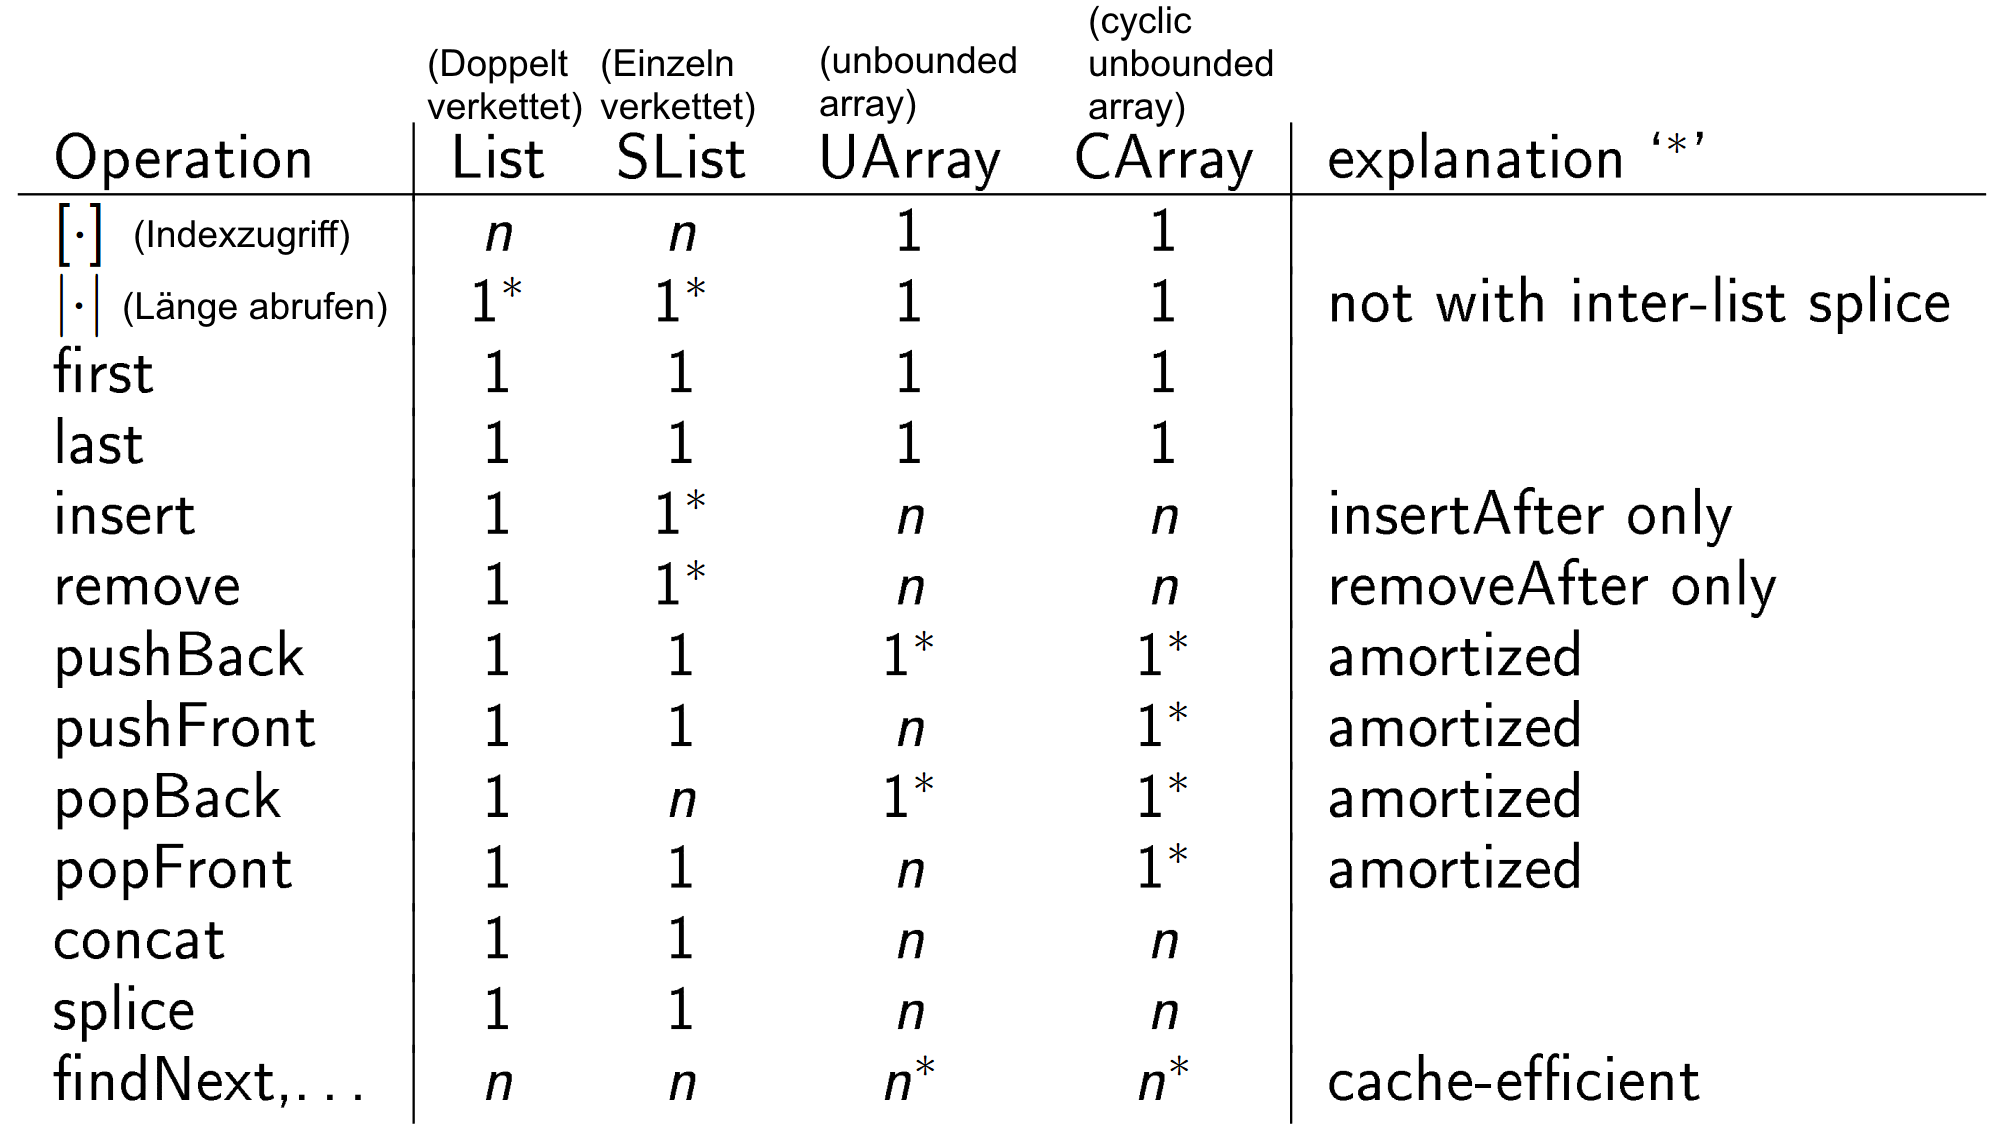
\includegraphics[height=6cm]{listenvsarrays}
	\end{figure}
\end{frame}

\begin{frame}{Listen und Co.}
	\taskheading{}
	Entwerft einen Stack, der $push$, $pop$ und $min$ kann und zwar in $O(1)$ (nicht amortisiert).
\end{frame}

\begin{frame}{Listen und Co.}
	\solutionheading
	\begin{algorithm}[H]
		$BasicStack, MinimumStack: Stack$ \;
		\;
		\Function{min}{
			\Return{$MinimumStack$.getTop} \;
		}
		\;
		\Procedure{push$(e)$}{
			$BasicStack$.push$(e)$ \;
			\lIf{$e \leq \text{min}$}{$MinimumStack$.push$(e)$}	
		}
		\;
		\Function{pop}{
			$r := BasicStack$.pop$()$ \;
			\lIf{$r = \text{min}$}{$MinimumStack$.pop$()$}	
			\Return{$r$}
		}
	\end{algorithm}
\end{frame}


\section{Hashing}

\begin{frame}{Hashing}
	\begin{itemize}
		\item \textbf{Erwartete} Laufzeit!
		\item \textbf{Hashfunktion} $h$ weist Elemente einem Platz in der Tabelle zu 
		\item \textbf{Universelle} Hashfunktionen \quad --- \quad  Vorlesung: \\
		Wenn $n \in O(m)$ Elemente in die Hashtable eingefügt werden \impl erwartete $\abs{\text{Kollisionen}} \in O(1)$ 
		\item Typische Familie univ. Hashfunktionen: \\
		$h_a(x) := a \cdot x \mod m \quad (0 < a < m)$ \quad ($m$ \textbf{prim}!)
		\item Oder generisch (z. B., falls in Klausur nötig): „Sei $h$ eine beliebige Hashfunktion aus der Familie universeller Hashfunktionen“
	\end{itemize}
	\bigskip
	\small Aufgaben: \\
	\hanging \emph{Konstruktion}: Probeklausur '17 A4, SS 2017 ÜB4 A1, Altklausuren 2015 A6b, 2010 A3, ... \\
	\emph{Op-Folge angeben}: Probeklausur '17 A2b, Altklausur 2010 A6a, ...
\end{frame}	

\begin{frame}{Hashing}	
	\textbf{Hashing mit verketteten Listen}
	\begin{itemize}
		\implitem Halte $\KwArrayOf \text{Lists}$: \\ 
		Werfe Element in die Liste, suche es dort
	\end{itemize}
	\pause
	\textbf{Hashing mit linearer Suche}
	\begin{itemize}
		\implitem Nur $\KwArrayOf \text{Element}$: \\
		Platz besetzt? Gucke rechts davon. \\
		Beim \textbf{Löschen}: Ggfs. wieder nach links zurückschieben, damit Lücken wieder zu!
		\item Ganz rechts im Array Platz dicht? \\
		\impl Pufferbereich (der dann hoffentlich langt)  \quad oder \\
		\impl Zyklisch 
	\end{itemize}
\end{frame}
	


\section{Sortieren}

\begin{frame}{Sortieralgorithmen}
	\textbf{Vergleichsbasiert}
	\begin{itemize}
		\item InsertionSort \hfill {\small (Elemente blubbern einzeln nach unten, bis sie passen)}
		\item (SelectionSort) \hfill {\small (Wähle nächstes passendes Element aus)}
		\item (BubbleSort) \hfill {\small (Elemente blubbern einzeln nach oben, bis sie passen)}
		\item Mergesort \hfill {\small (Listen mehrmals halbieren, dann zurückmergen)}
		\item Quicksort \hfill  {\small („Pivot-Vorsortierung“, Teile rekursiv weitersortieren)} 
		\item Heapsort (\textbf{ab}steigende Sortierung!) \hfill {\small (baue Heap auf, $n$-mal $deleteMin$)}  
	\end{itemize}
	\textbf{Ganzzahlig}
	\begin{itemize}
		\item BucketSort \hfill {\small (Elemente in passenden „Eimer“ werfen)}
		\item CountingSort \hfill {\small (Anzahl zählen statt reinzuwerfen)}
		\item LSD-RadixSort \hfill {\small (nach den einzelnen Ziffern sortieren)}
	\end{itemize}
\end{frame}

\begin{frame}{Sorting Algorithms}
	\textbf{Sortiere} Mergesort, Radixsort, Heapsort, InsertionSort, SelectionSort, CountingSort, Quicksort {\small (mit partition)}, (simples) Bucketsort nach \textbf{Stabilität}. \\ \pause
	\forcenewline
	\centering
	\begin{tabular}{m{.3\linewidth} | m{.2\linewidth} |}
		\hline
		InsertionSort \newline 
		SelectionSort \newline
		Mergesort \newline
		CountingSort \newline
		Bucketsort \newline
		Radixsort & \YesCell \\
		\hline
		Heapsort \newline
		Quicksort & \NoCell \\
		\hline
	\end{tabular}
\end{frame}

\begin{frame}{Sorting Algorithms}
	\textbf{Sortiere} Mergesort, Radixsort, Heapsort, InsertionSort, SelectionSort, CountingSort, Quicksort {\small (mit partition)}, (simples) Bucketsort nach \textbf{Cache-Effizienz}. \\ \pause
	\forcenewline
	\centering
	\begin{tabular}{m{.3\linewidth} | m{.2\linewidth} |}
		\hline
		InsertionSort \newline 
		SelectionSort \newline
		Heapsort \newline
		CountingSort \newline
		Quicksort & \YesCell \\
		\hline
		Bucketsort \newline
		Mergesort \newline
		Radixsort & \NoCell \\
		\hline
	\end{tabular}
\end{frame}

\begin{frame}{Sorting Algorithms}
	\textbf{Sortiere} Mergesort, Radixsort, Heapsort, InsertionSort, SelectionSort, CountingSort, Quicksort {\small (mit partition)}, (simples) Bucketsort nach \textbf{Platzverbrauch}. \\ \pause
	\forcenewline
	\centering
	\begin{tabular}{m{.55\linewidth} | m{.15\linewidth} }
		\hhline{=|=}
		InsertionSort \newline 
		SelectionSort \newline
		Mergesort (ohne Rekursionsoverhead) \newline
		Quicksort (ohne Rekursionsoverhead) & $O(1)$ \\
		\hline
		Heapsort & $O(n)$ \\
		\hhline{=|=}
		CountingSort \newline 
		Bucketsort & $O(n+k)$ \\
		\hhline{=|=}
		Radixsort & $O(n+K)$ \\
		\hhline{=|=}
	\end{tabular}
\end{frame}

\begin{frame}{Sorting Algorithms}
	\textbf{Sortiere} Mergesort, Radixsort, Heapsort, InsertionSort, SelectionSort, CountingSort, Quicksort {\small (mit partition)}, (simples) Bucketsort nach \textbf{Worst-Case-Laufzeit}. \\ \pause
	\forcenewline
	\begin{columns}
		\column{.45\textwidth}
		\begin{tabular}{m{.4\linewidth} | m{.3\linewidth} }
			\hhline{=|=}
			Mergesort \newline
			Heapsort & $O(n \log n)$ \\
			\hline
			Quicksort \newline 
			InsertionSort \newline 
			SelectionSort & $O(n^2)$ \\
			\hhline{=|=}
		\end{tabular}
		\column{.45\textwidth}
		\hspace{-2\baselineskip}
		\begin{tabular}{m{.37\linewidth} | m{.47\linewidth} }
			\hhline{=|=}
			Radixsort & $O(d \cdot (n + K))$ \newline ($K$: Basis, \newline $d$: Digits)\\
			\hhline{=|=}
			Bucketsort \newline
			Countingsort & $O(n+k)$ \newline ($k$: „maxValue“) \\
			\hhline{=|=}
		\end{tabular}
	\end{columns}
\end{frame}

\begin{frame}{Sorting Algorithms}
	\textbf{Sortiere} Mergesort, Radixsort, Heapsort, InsertionSort, SelectionSort, CountingSort, Quicksort {\small (mit partition)}, (simples) Bucketsort nach \textbf{„Standard-Laufzeit“}. \\ \pause
	\forcenewline
	\begin{columns}
		\column{.55\textwidth}
		\hspace{.2\baselineskip}
		\begin{tabular}{m{.487\linewidth} | m{.3\linewidth} }
			\hhline{=|=}
			Mergesort \newline
			Heapsort \newline 
			Quicksort (erwartet) & $O(n \log n)$ \\
			\hline 
			InsertionSort \newline 
			SelectionSort & $O(n^2)$ \\
			\hhline{=|=}
		\end{tabular}
		\column{.45\textwidth}
		\hspace{-1\baselineskip}
		\begin{tabular}{m{.37\linewidth} | m{.47\linewidth} }
			\hhline{=|=}
			Radixsort & $O(d \cdot (n + K))$ \newline ($K$: Basis, \newline $d$: Digits)\\
			\hhline{=|=}
			Bucketsort \newline
			Countingsort & $O(n+k)$ \newline ($k$: „maxValue“) \\
			\hhline{=|=}
		\end{tabular}
	\end{columns}
\end{frame}




\section{Binäre Heaps / Sortierte Folgen}

\begin{frame}{Binäre Heaps}
	\textbf{Implementierung} \\
	\begin{itemize}
		\item Repräsentiere binären Baum als $\KwArray[1...n]$ mit \textbf{Heap-Eigenschaft}
		%
		\item Die Ebenen des Baumes liegen von \textbf{oben $\rightsquigarrow$ unten} und \\ von \textbf{links $\rightsquigarrow$ rechts} nacheinander im Array 
		
		\item Von Knoten $j$ kriegt man \textbf{Eltern} und \textbf{Kinder} wie folgt:
	\end{itemize}

	\begin{columns}
		\column{.4\textwidth}
		\vspace{-7\baselineskip} % [T] option doesn't even work. Fuck you, LaTeX!
		\begin{align*}
		&parent(j) = \floor{\tfrac{j}{2}} \\
		&leftChild(j) = 2j \\
		&rightChild(j) = 2j + 1
		\end{align*}
		
		\column[c]{.5\textwidth}
		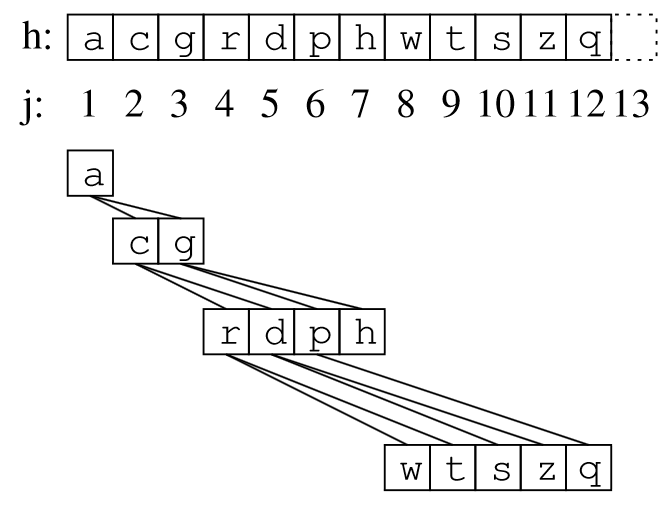
\includegraphics[height=4.7cm]{heaparray}
	\end{columns}
\end{frame}

\begin{frame}{Binäre Heaps}
	\begin{itemize}
		\item $insert$: Nach unten rechts und \emph{siftUp}
		\item $deleteMin$: Element ganz unten rechts \~~> ganz oben, \emph{siftDown}
		\item $buildHeap$: „Ebenen“ von unten \~~> oben durchgehen und „down-siften“, dass es passt \quad in $O(n)$
	\end{itemize}
\end{frame}





\begin{frame}{Sortierte Folgen -- (a, b)-Bäume}
	\textbf{Beispiel: (2, 4)-Baum} („00“ steht in VL für $\infty$) \\[0,125cm]
	\begin{figure}[htp]
		\centering
		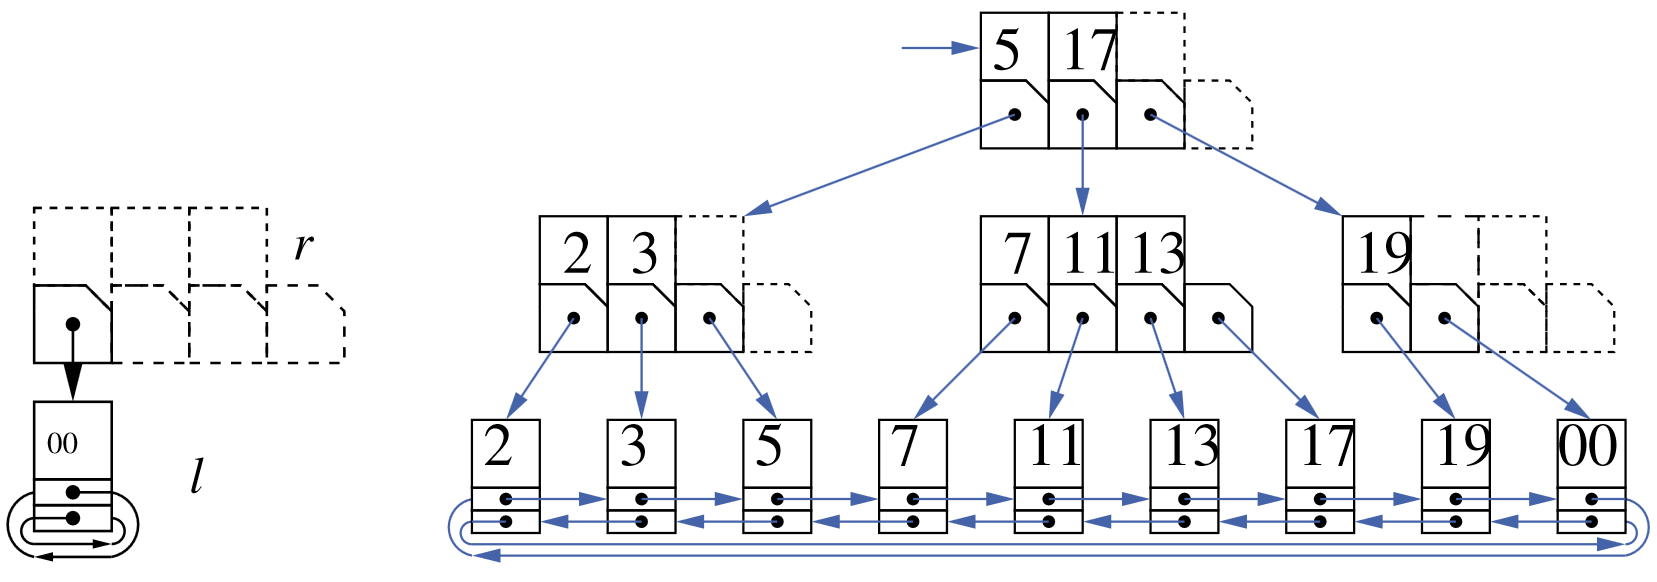
\includegraphics[width=\textwidth]{baum24}
	\end{figure}
\end{frame}



\section{Graphen}

\begin{frame}{Graphen}
	\textbf{Repräsentationen} 
	\pause
	\begin{itemize}
		\item Kantenfolge
		\item Adjazenzmatrix
		\item Adjazenzfeld
		\item Adjazenzliste
	\end{itemize}
	
	\textbf{Durchlaufen}
	\begin{itemize}
		\item Tiefensuche
		\item Breitensuche
		\implitem Kantenklassifikation
	\end{itemize}
	
	\bigskip
	\small
	Aufgaben: \\
	\emph{Konstruktion}: Altklausur 2010 A1a, ... \\
	\emph{BFS anwenden, sodass}: Altklausur 2010 A1f, ...\\
\end{frame}

\begin{frame}{Graphen}
	\textbf{Kürzeste Wege}
	\begin{tabular}{rll}
		Dijkstra &  Kantengewichte $\geq 0$, & $O((m+n) \log n)$ \\
		Bellman-Ford & Kantengew. $\in \R$, erkennt neg. Zyklen, & $O(n \cdot m)$ 
	\end{tabular} \\
	\smallskip
	\hfill {\tiny Aufgaben: \emph{Anwenden} (Altk. 2010 A2, 2013 A2a), \emph{Theorie} (Altk. 2013 A2c), ...} \\
	\pause
	\textbf{Minimale Spannbäume}
	\begin{itemize}
		\item \emph{Schnitteigenschaft}: \textbf{Leichteste} Kante in nem Schnitt: Nehmen!
		\item \emph{Kreiseigenschaft}: \textbf{Schwerste} Kante in nem Kreis: Raus!
		\implitem \emph{Jarník-Prim}: Dijkstra-ähnlich – Aufspannen
		\implitem \emph{Kruskal}: Kanten von leicht \~~> schwer hinzufügen, wenn's geht
	\end{itemize}
	\hfill {\tiny Aufgaben: \emph{Anwenden} (Altk. 2010 A5a, 2015 A2b, 2014 A6b), ...} \\
	\pause
	\textbf{Union-Find} (für Kruskal)
	\begin{itemize}
		\item Kleine Bäumchen repräsentieren zusammenhäng. \textbf{Knoten}mengen
		\item Pfadkompression
		\item Union-By-Rank
	\end{itemize}
\end{frame}


\section{Optimierungsprobleme}

\begin{frame}{Optimierungsprobleme}
	\textbf{Ansätze:}
	\begin{itemize}
		\item Greedy
		\item DP
		\item[...] (s. VL)
		\item ILPs
	\end{itemize}
	\forcenewline
	{\small Aufgaben: 
		\begin{itemize}
			\item Altklausur 2014\_2 A3 „MaxSubArray“;
			\item Münzproblem (SS~2016 Übung~12 Folie~5 \\ {\footnotesize \url{http://crypto.iti.kit.edu/fileadmin/User/Lectures/Algorithmen\_SS16/ue12-slides.pdf}})
			\item Altklausur 2016\_2 A5 „Chemie-ILP“
		\end{itemize}
	}
\end{frame}





%%%%%%%%%%%%%%%%%%%%%%%%%%%%%%%%%%%%%%%%%%%%%%%%%%%%%%%%%%%%%%%%%%%%%%%

	
\begin{headframe}[Ihr wart ein tolles Tut. \smiley \\ \small Questions? \~~> Mail me!]
	Danke fürs Dasein und \\
	viel Glück für eure Klausuren! \smiley 
\end{headframe}
	

\end{document}